\documentclass[10pt,letterpaper]{article}
%\usepackage{times}
\usepackage[margin=1in,hmargin=1in]{geometry}
\usepackage{amsmath}
\usepackage{tikz,url}
\usepackage{amssymb}
\usepackage{fancyhdr}
\usetikzlibrary{matrix}
\usepackage{listings}
\usepackage{tabularx}
\usepackage{xcolor}
\usepackage{graphicx}
\usepackage{graphics}
\usepackage{titling}
\pagestyle{fancy}
\usepackage{float}
\usepackage{fancyvrb}
\usepackage{verbatim}
\usepackage{enumitem}
\usepackage{alltt}
\usepackage{pdfpages}
%\usepackage{float}
%\restylefloat{table}

\fancyhead[LO]{STAT W4201 Advanced Data Analysis}
\fancyhead[RO]{HW 1}
\fancyhead[LE]{STAT W4201 Advanced Data Analysis}
\fancyhead[RE]{HW 1}
\title{\textbf {Homework 1}}
\author{{Qianbo Wang}\\{uni: qw2180}}
\date{}
\setlength{\droptitle}{-5em}
\setlength{\parindent}{0pt}

\makeatletter
\newcommand{\rmnum}[1]{\romannumeral #1}
\newcommand{\Rmnum}[1]{\expandafter\@slowromancap\romannumeral #1@}
\makeatother
\lstset{
language=R,
tabsize=4, 
commentstyle=\color{red!50!green!50!blue!50},
keywordstyle=\color{blue!90},
showstringspaces=false,
stringstyle=\ttfamily,
keepspaces=true, 
breakindent=22pt, 
stepnumber=1,
numberstyle={\color[RGB]{0,192,192}\tiny} ,
numbersep=5pt,  
basicstyle=\footnotesize,
showspaces=false, 
flexiblecolumns=true, 
comment=[l]{\#},
texcl=true,
escapeinside={\$$}{\^^M},
breaklines=true, 
breakautoindent=true,
breakindent=4em, 
aboveskip=1em, 
tabsize=2,
showstringspaces=false, 
backgroundcolor=\color[RGB]{244,244,244}, 
fontadjust,
captionpos=t,
framextopmargin=2pt,framexbottommargin=2pt,abovecaptionskip=-3pt,belowcaptionskip=3pt,
extendedchars=false,columns=flexible,
}

\begin{document}
\maketitle
\thispagestyle{fancy}
\vspace{-2em}
\textbf{Consider the Salary Data (Display 1.3) in Ramsey \& Schafer. Chapter 1, and partially appended below.}
\begin{enumerate}[leftmargin=0cm,itemindent=.5cm,labelwidth=\itemindent,labelsep=0cm,align=left]
\item[\Rmnum{1}). ] Determine whether there are outliers in the combined data, using boxplots or other suitable methods.

From the box-plot below, we can find that within the combined data for salary. There is one outlier here with salary 8100 and sex MALE.
\begin{center}
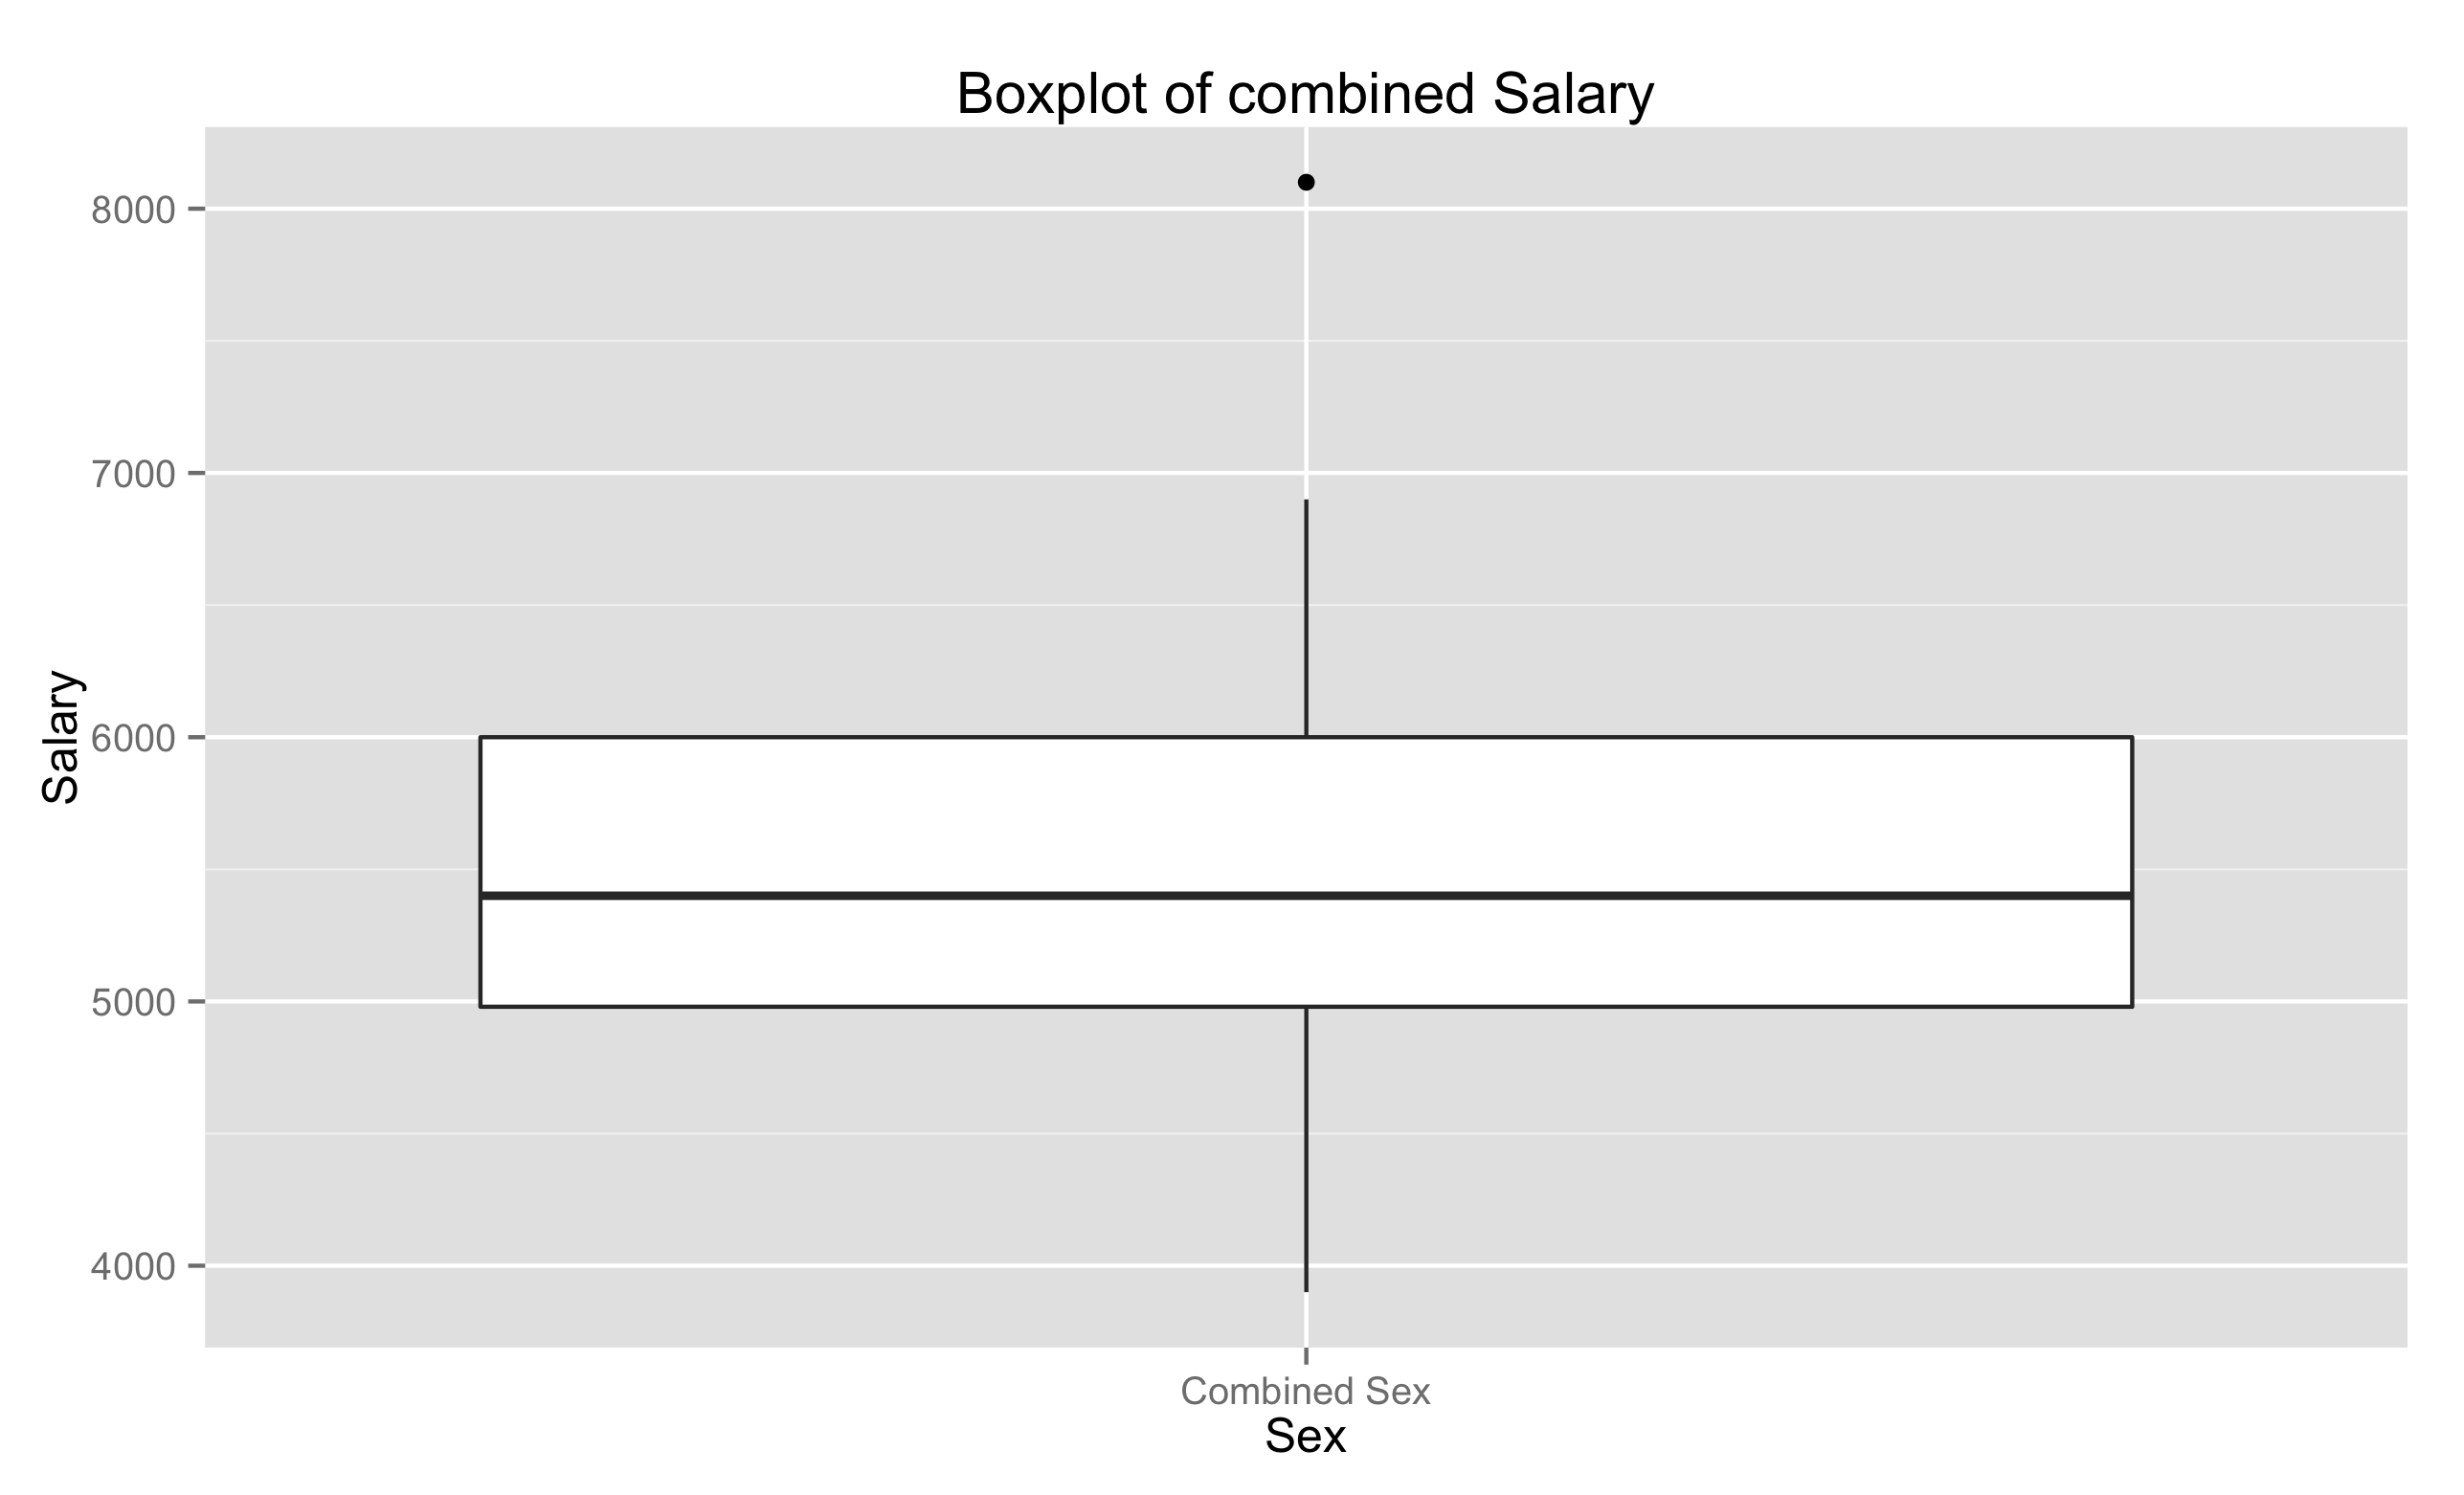
\includegraphics[scale=0.13]{boxcombined}
\end{center}

We can also see from the stem-leaf plot that there is an outlier in the combined data. 
\begin{center}
stem-leaf plot for combined data
\verbatiminput{stemCombined.txt}
\end{center}

\item[\Rmnum{2}). ] Performs seperate EDA, and compute the sample SD and IQR for Salary in each group.

First, check if there is missing value in data. We can find there is no missing values here because R function returns TRUE here.\\
Second, check if there is outlier here, from the grouped scatter-plot and box-plot we can find that there is one outlier within MALE group, which is of salary $8100$, whereas there is no outlier within FEMALE group. And from the first question we know that it is also the combined outlier.\\
And we can also see from the stem-leaf plot that there is an outlier in the MALE data, but no outlier in FEMALE data. \\
Third, draw histogram to see the number of observations in each group. MALE group has $32$ observations and FEMALE group has $61$ observations, with total $93$ observations. And also some other statistics, see the following table.\\
Fourth, draw estimate density plot to see the distribution. We can see that both of the two groups are not gaussian distribution but a little bit close gaussian.\\
Then, draw Q-Q plot to see the gaussian assumption. We can see that both of the two groups are not gaussian distribution.\\
And then, calculate the sample standard deviation. Sample SD in MALE group is  $690.7333$ and Sample SD in Female group is $640$.

\begin{table}
\caption{Statistic of FEMALE groups}
\centering
\begin{tabular*}{0.6\linewidth}{@{\extracolsep{\fill}}cccccc}
\hline 
Min & $1^{st}$qu & Median & Mean & $3^{rd}$qu & Max\\
\hline
3900 &4800 &5220 &5139 &5400 &6300\\
\hline
\end{tabular*}

\caption{Statistic of MALE groups}
\centering
\begin{tabular*}{0.6\linewidth}{@{\extracolsep{\fill}}cccccc}
\hline Min & $1^{st}$qu & Median & Mean & $3^{rd}$qu & Max\\
\hline
4620 &5400 &6000 & 5957 & 6075 &8100\\
\hline
\end{tabular*}

\caption{SD \& IQR}
\centering
\begin{tabular*}{0.6\linewidth}{@{\extracolsep{\fill}}ccc}
\hline &Sample SD & IQR\\
\hline
MALE & 690.7333 & 675\\
\hline
FEMALE & 539.8707 & 600\\
\hline
\end{tabular*}
\end{table}

\begin{center}
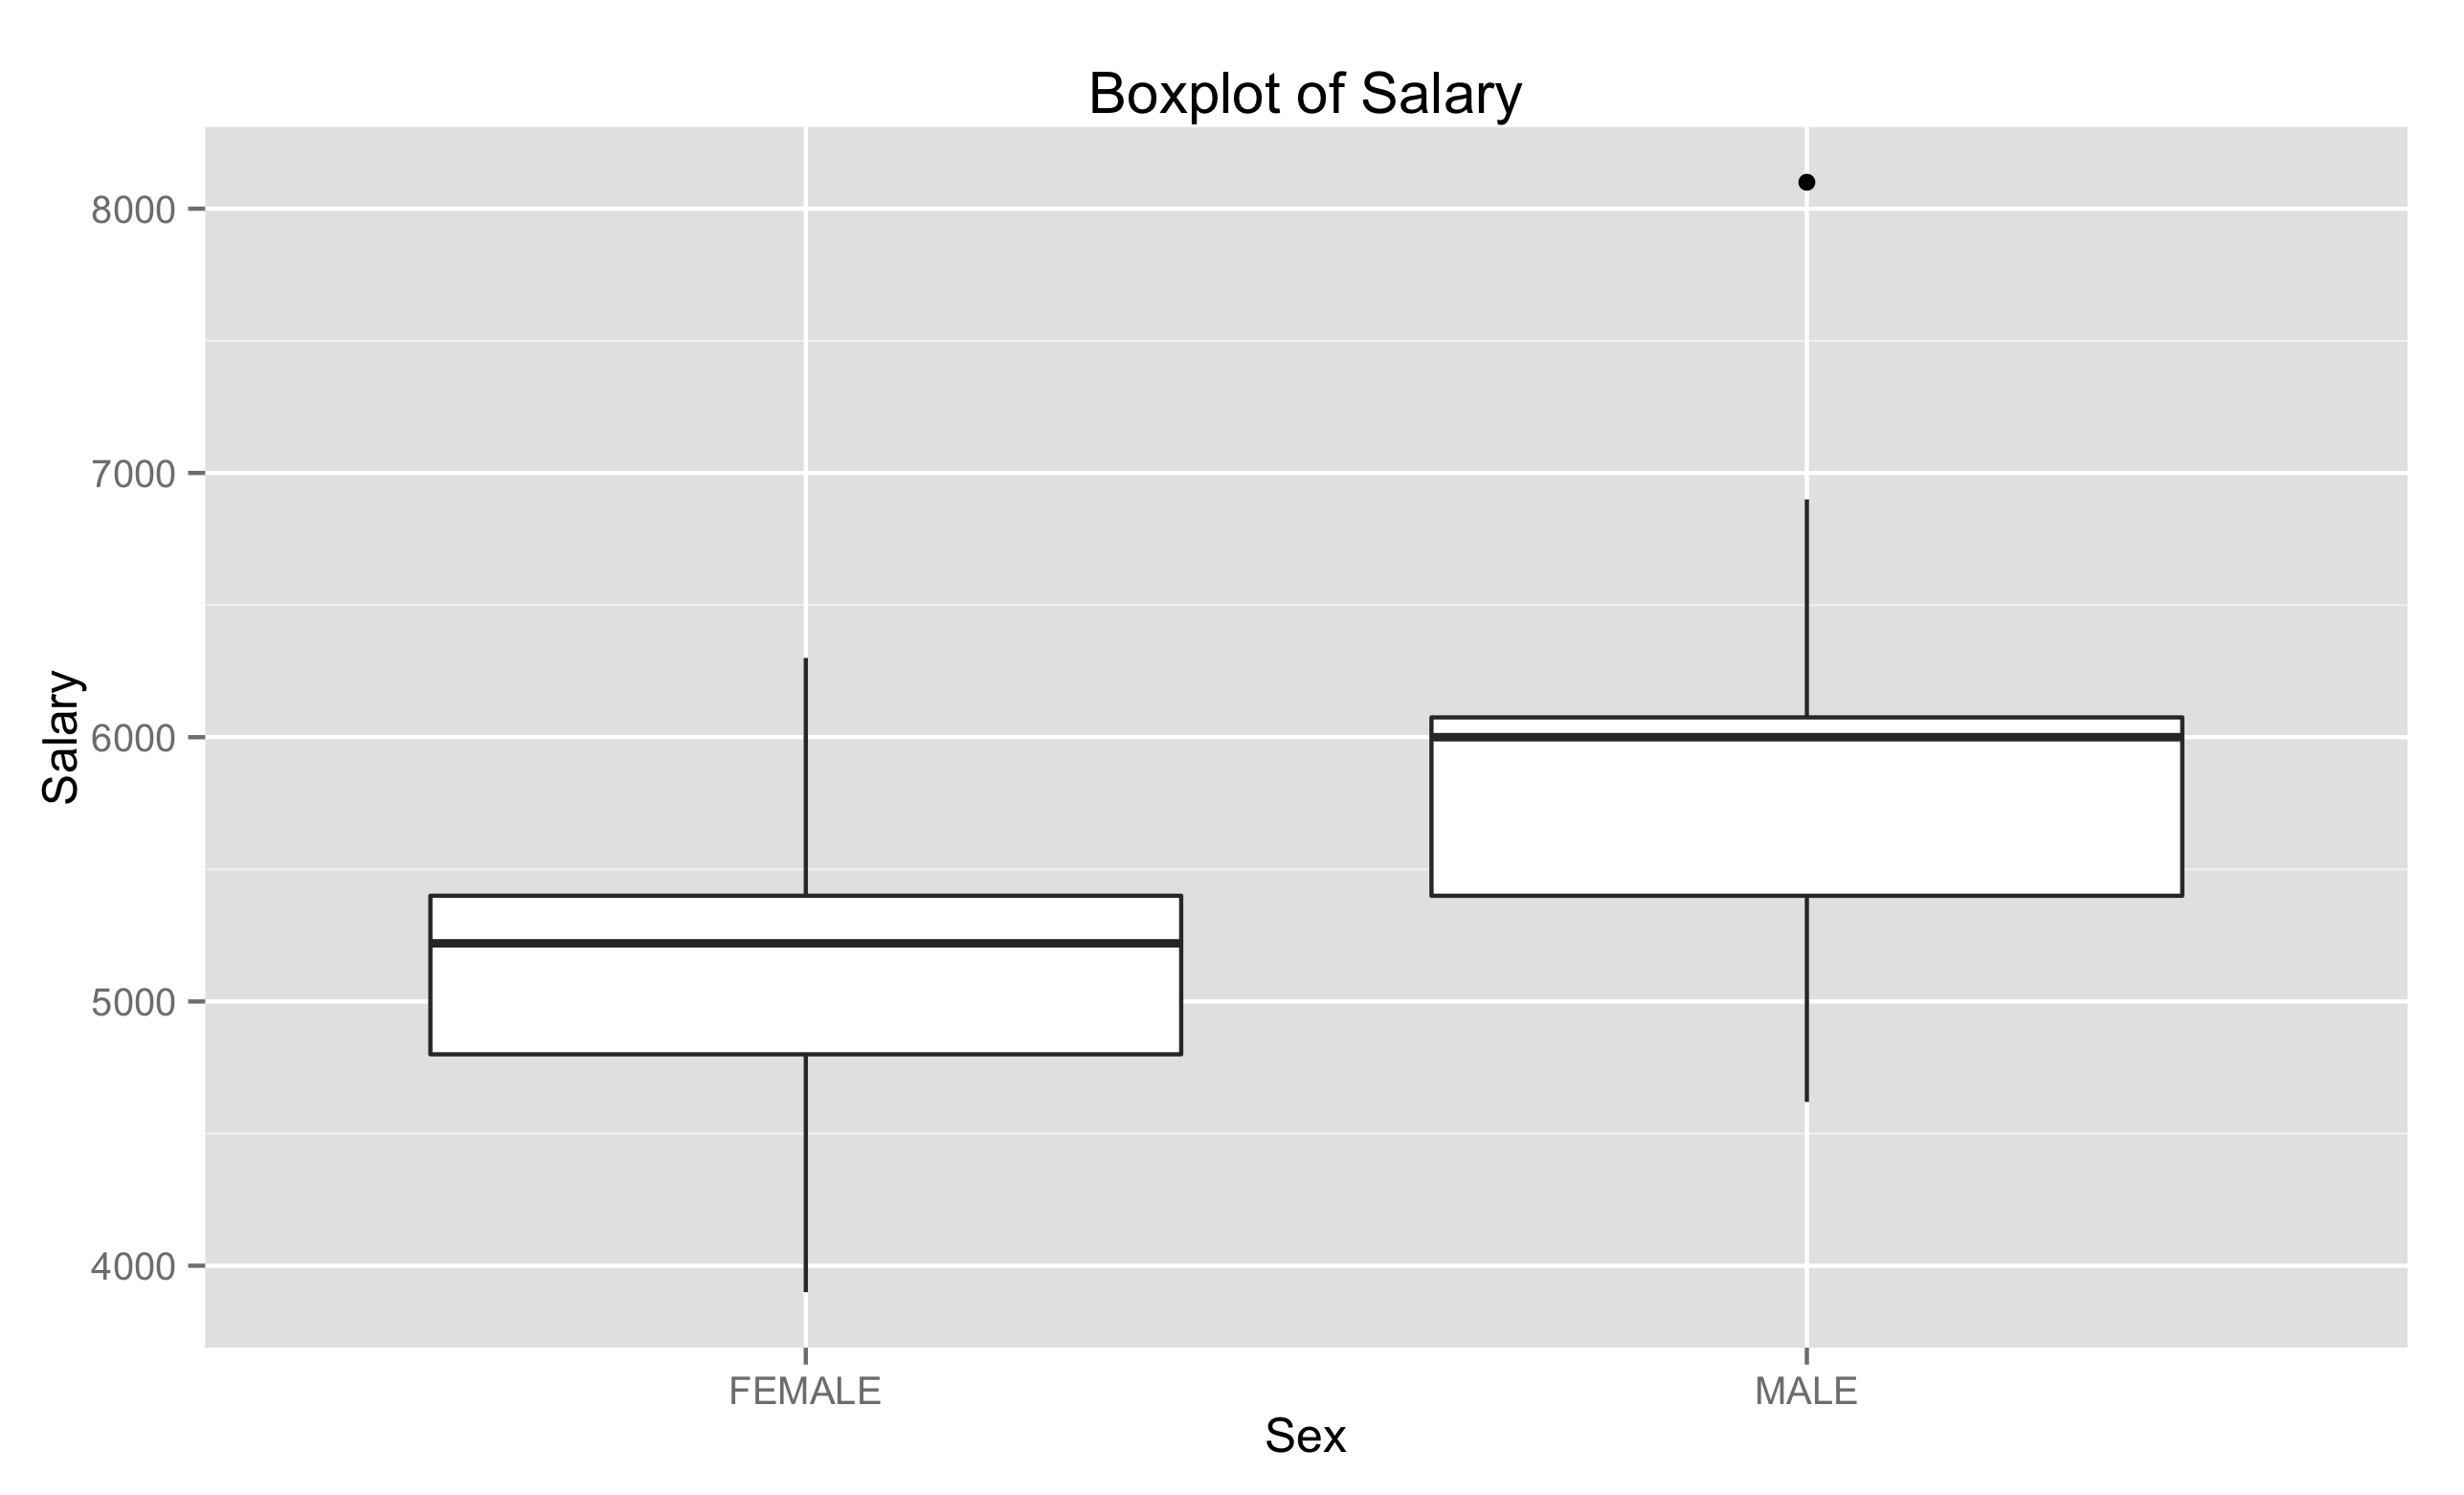
\includegraphics[scale=0.13]{boxgroup}
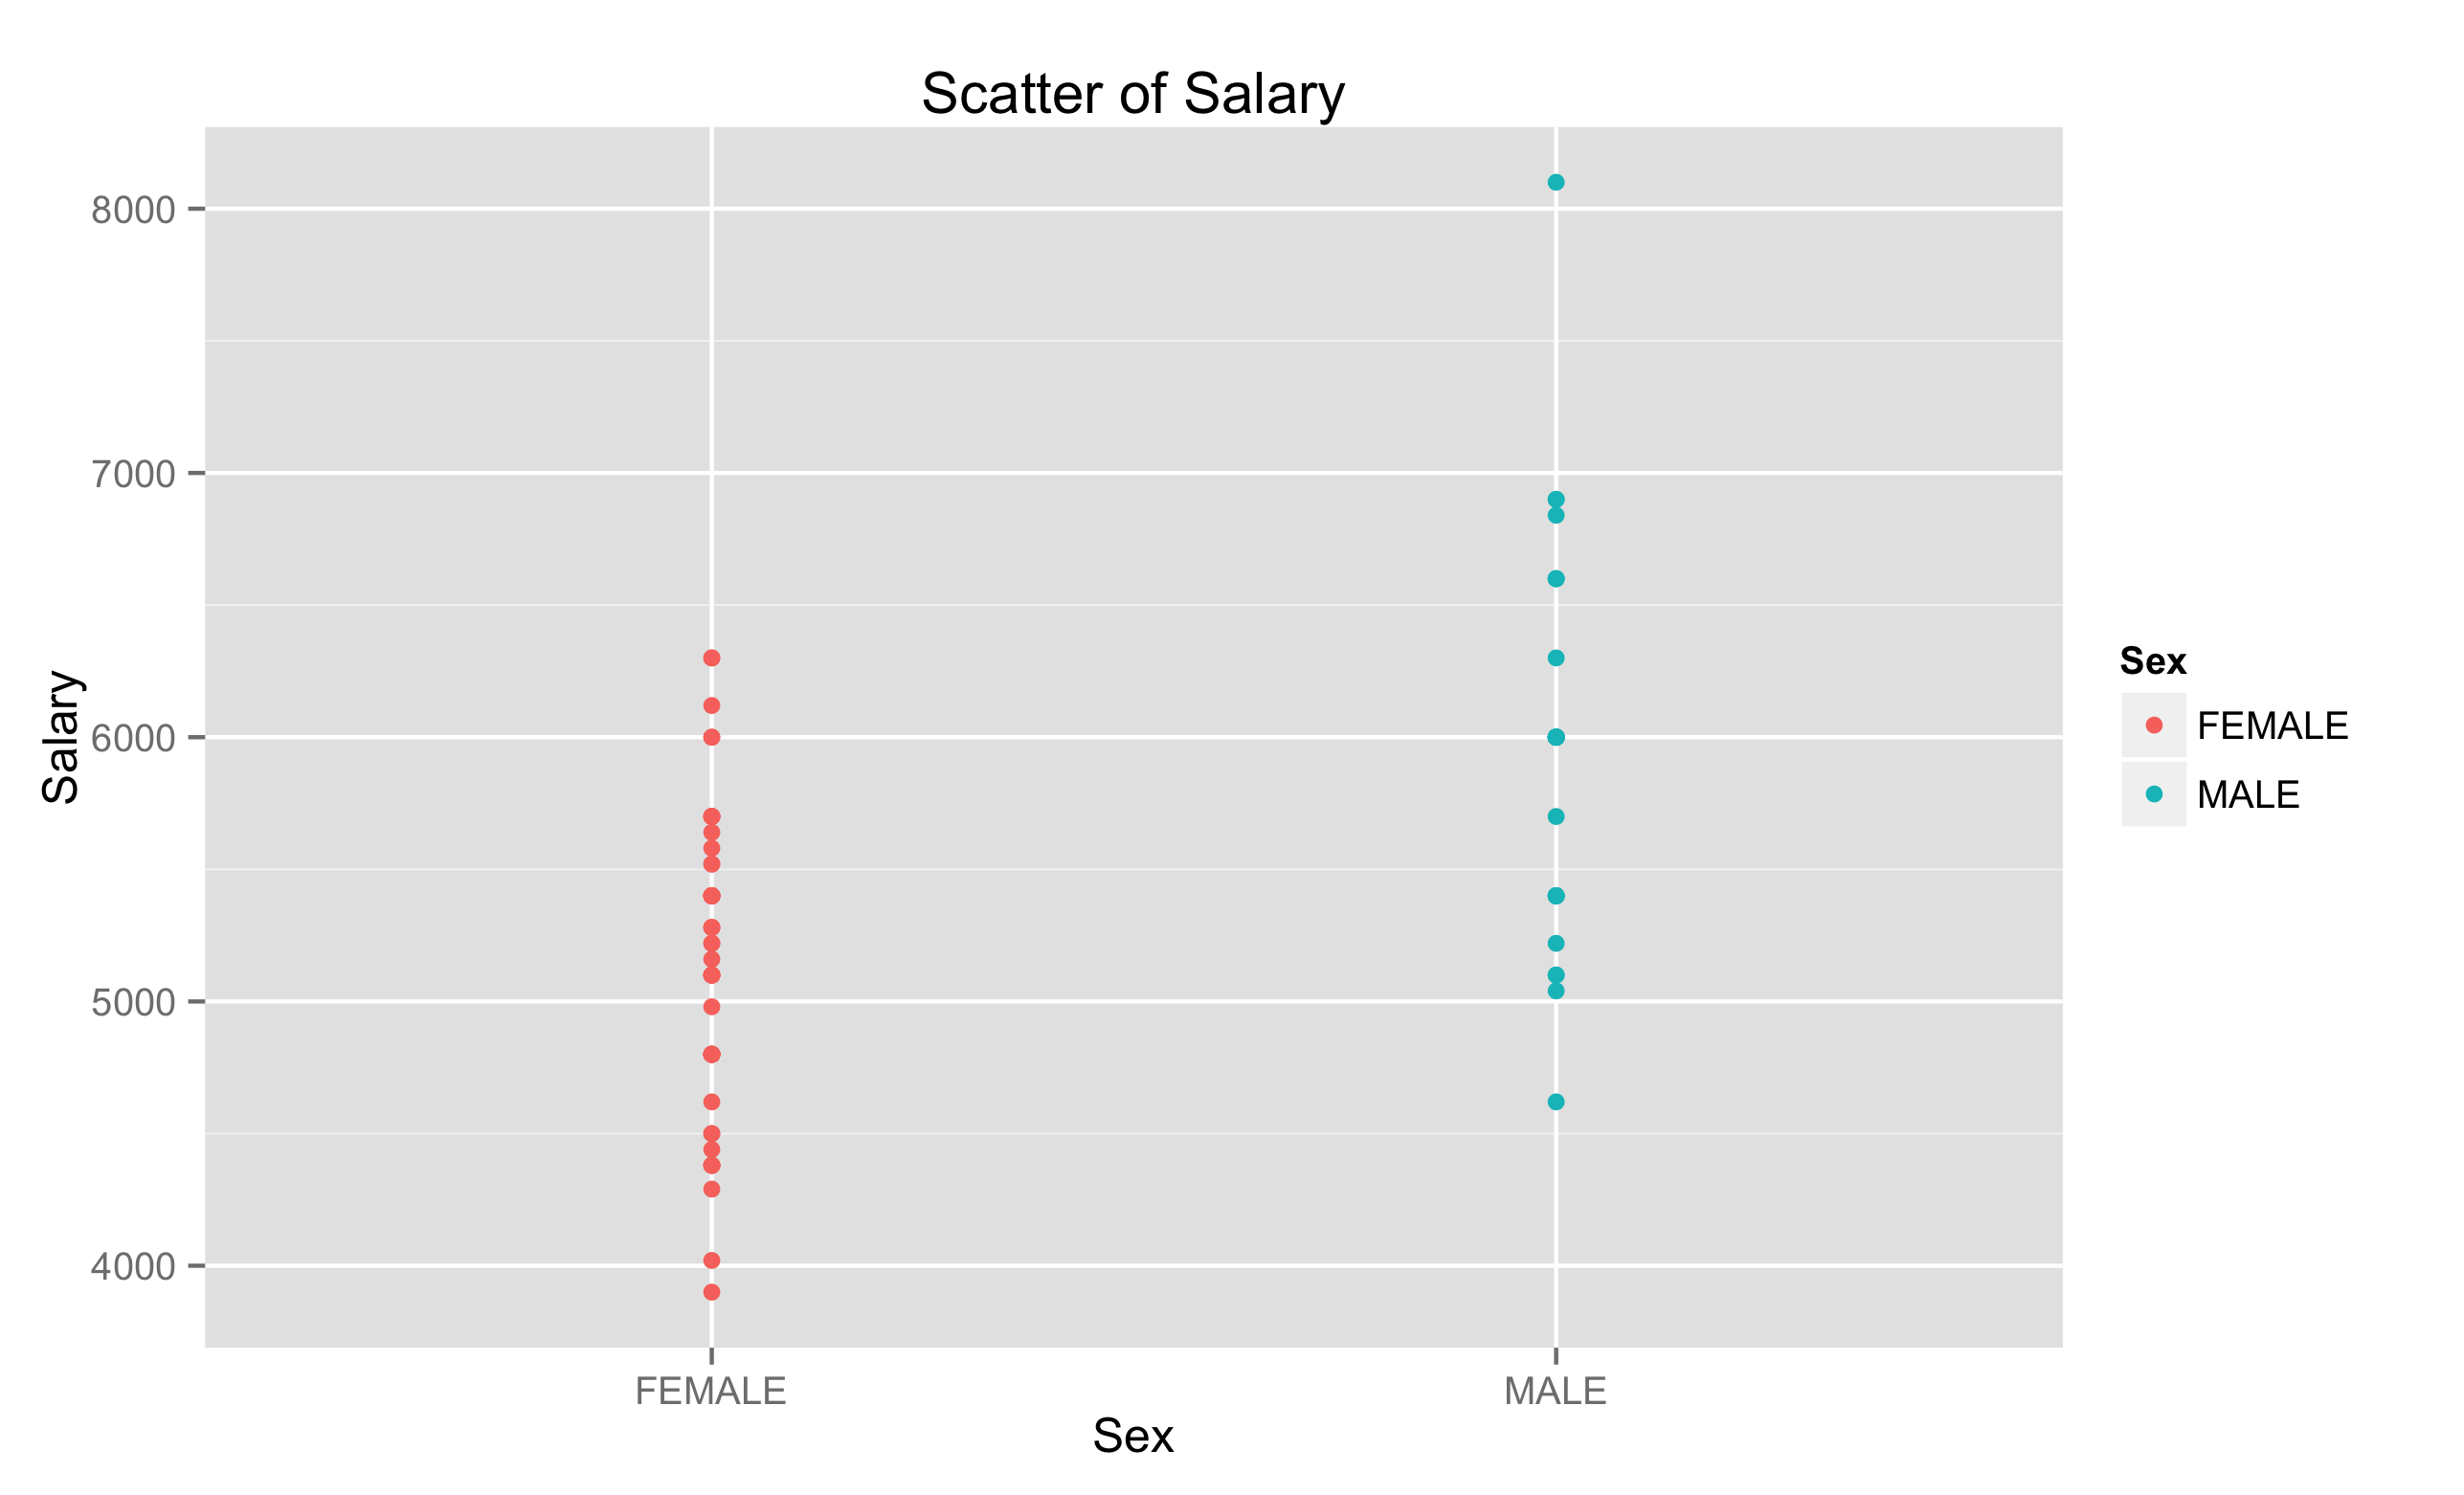
\includegraphics[scale=0.13]{scatter}
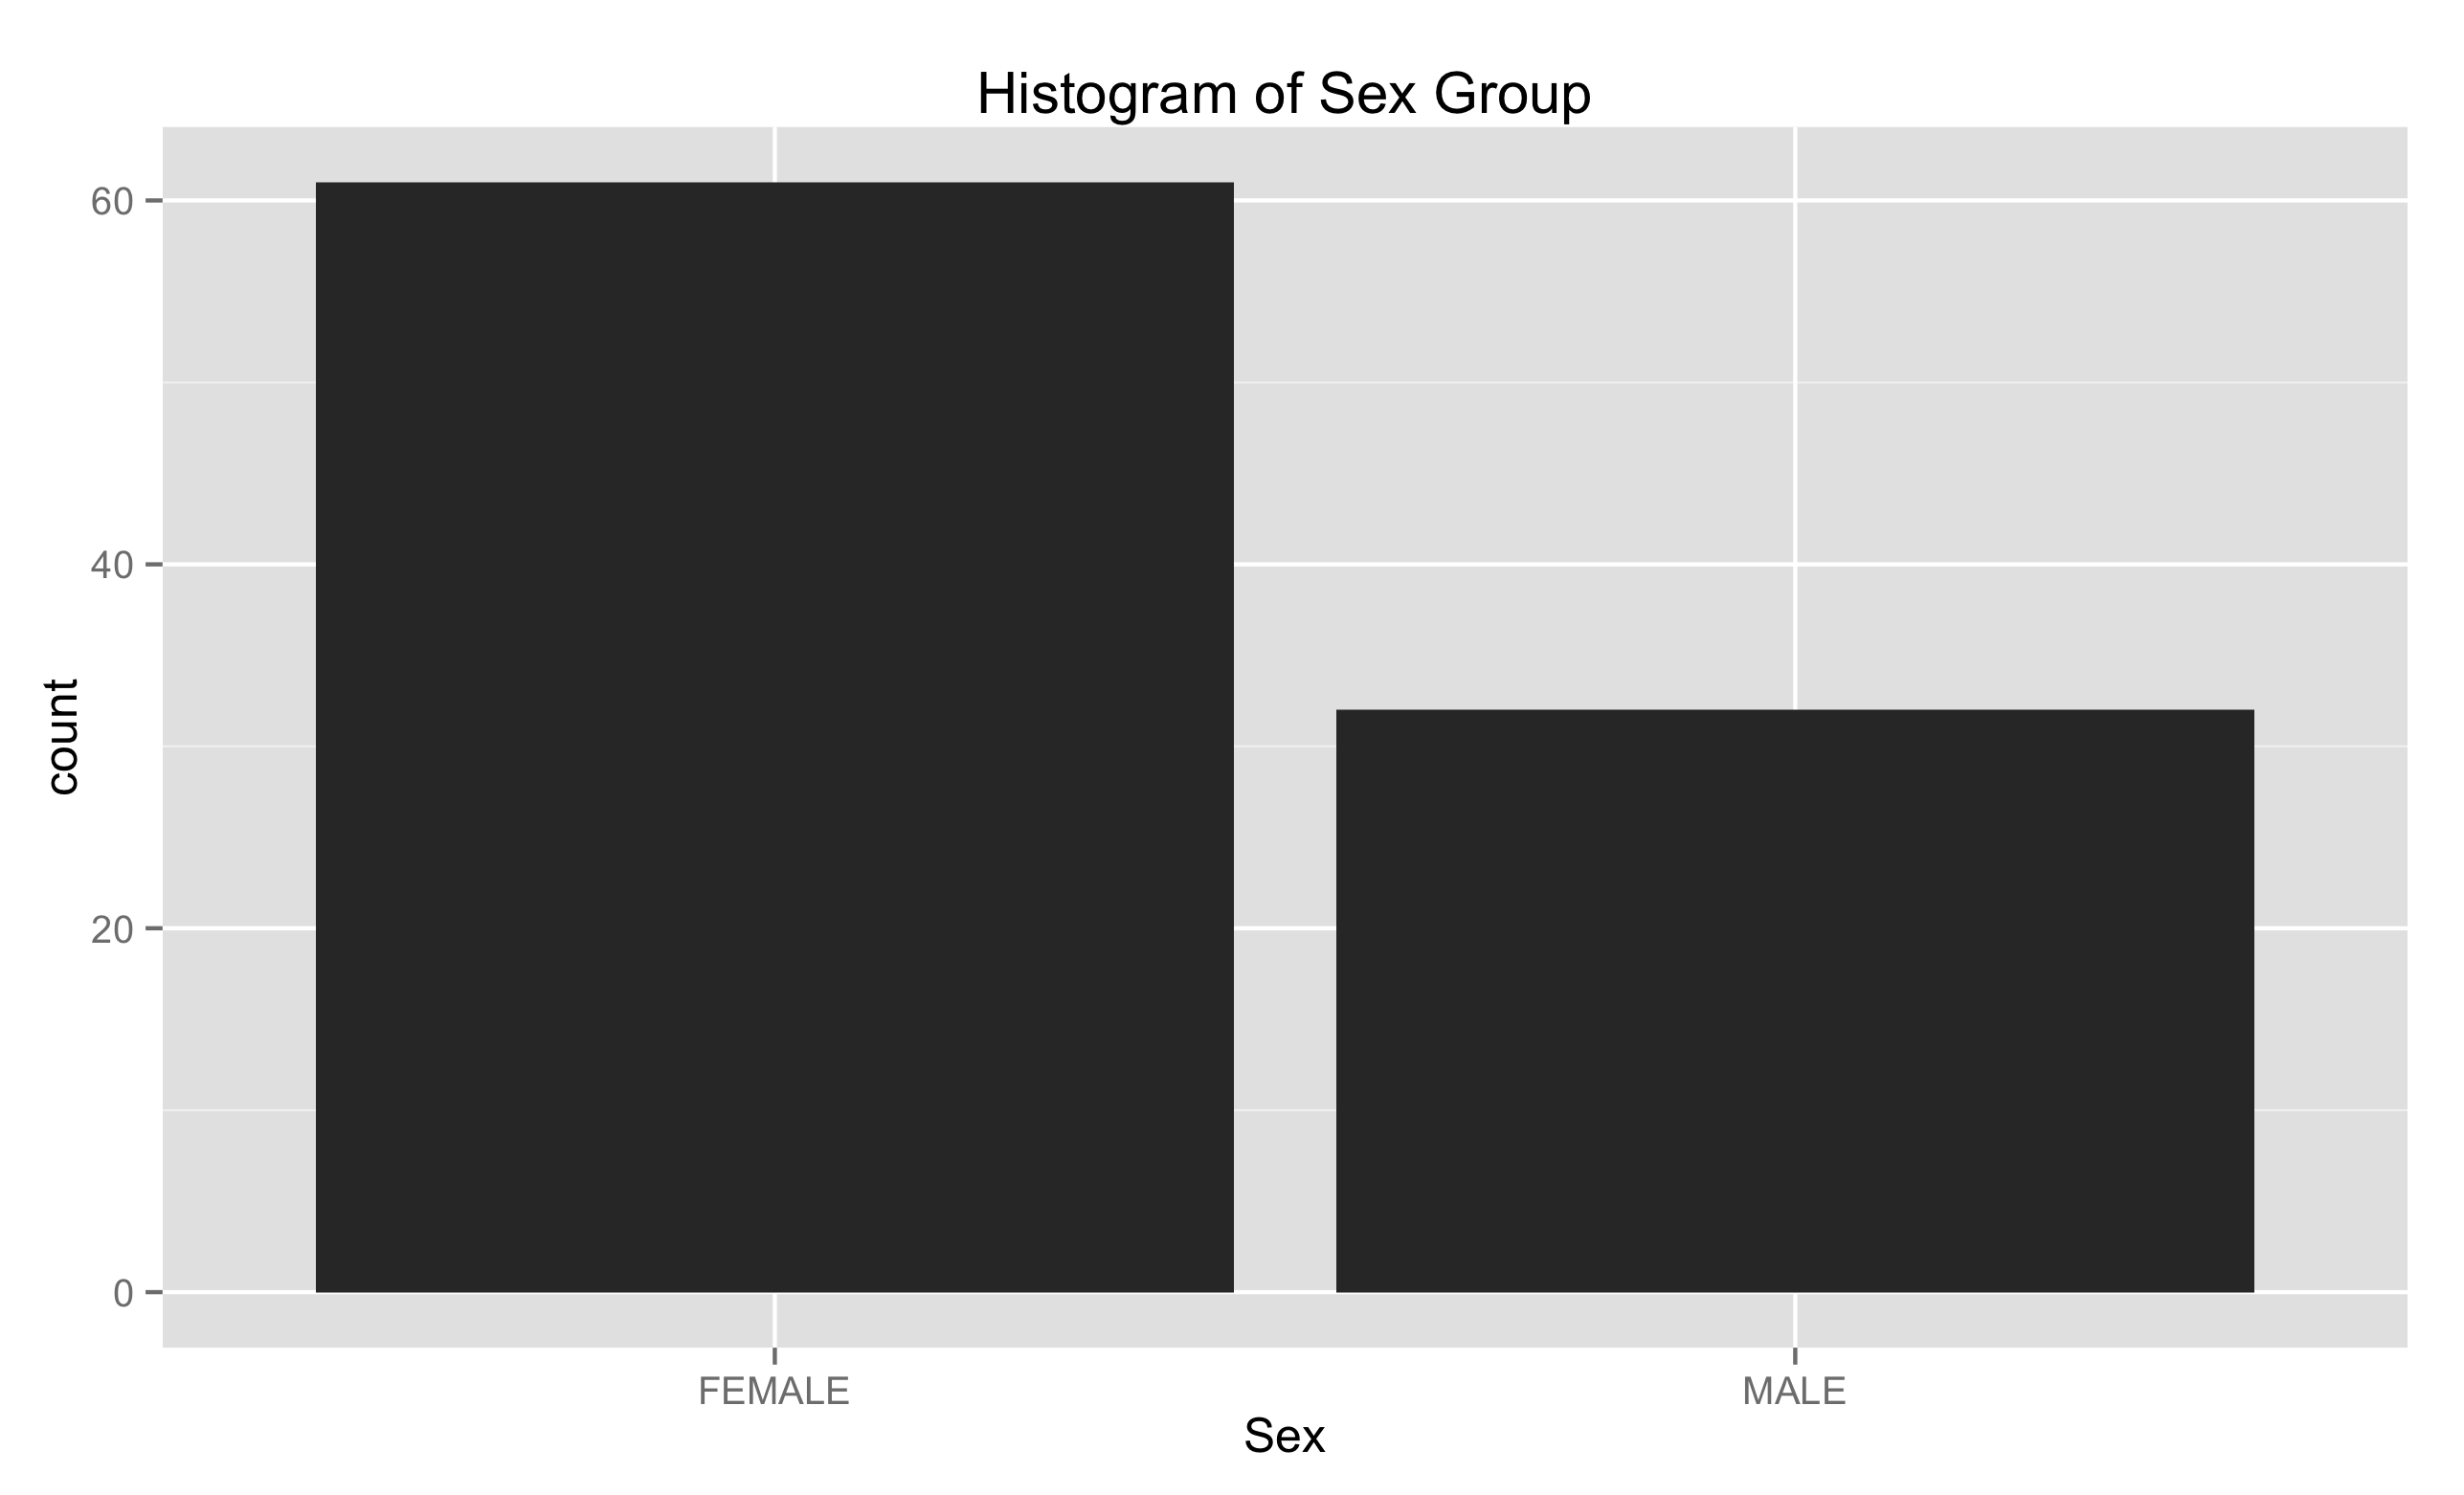
\includegraphics[scale=0.13]{histogram}
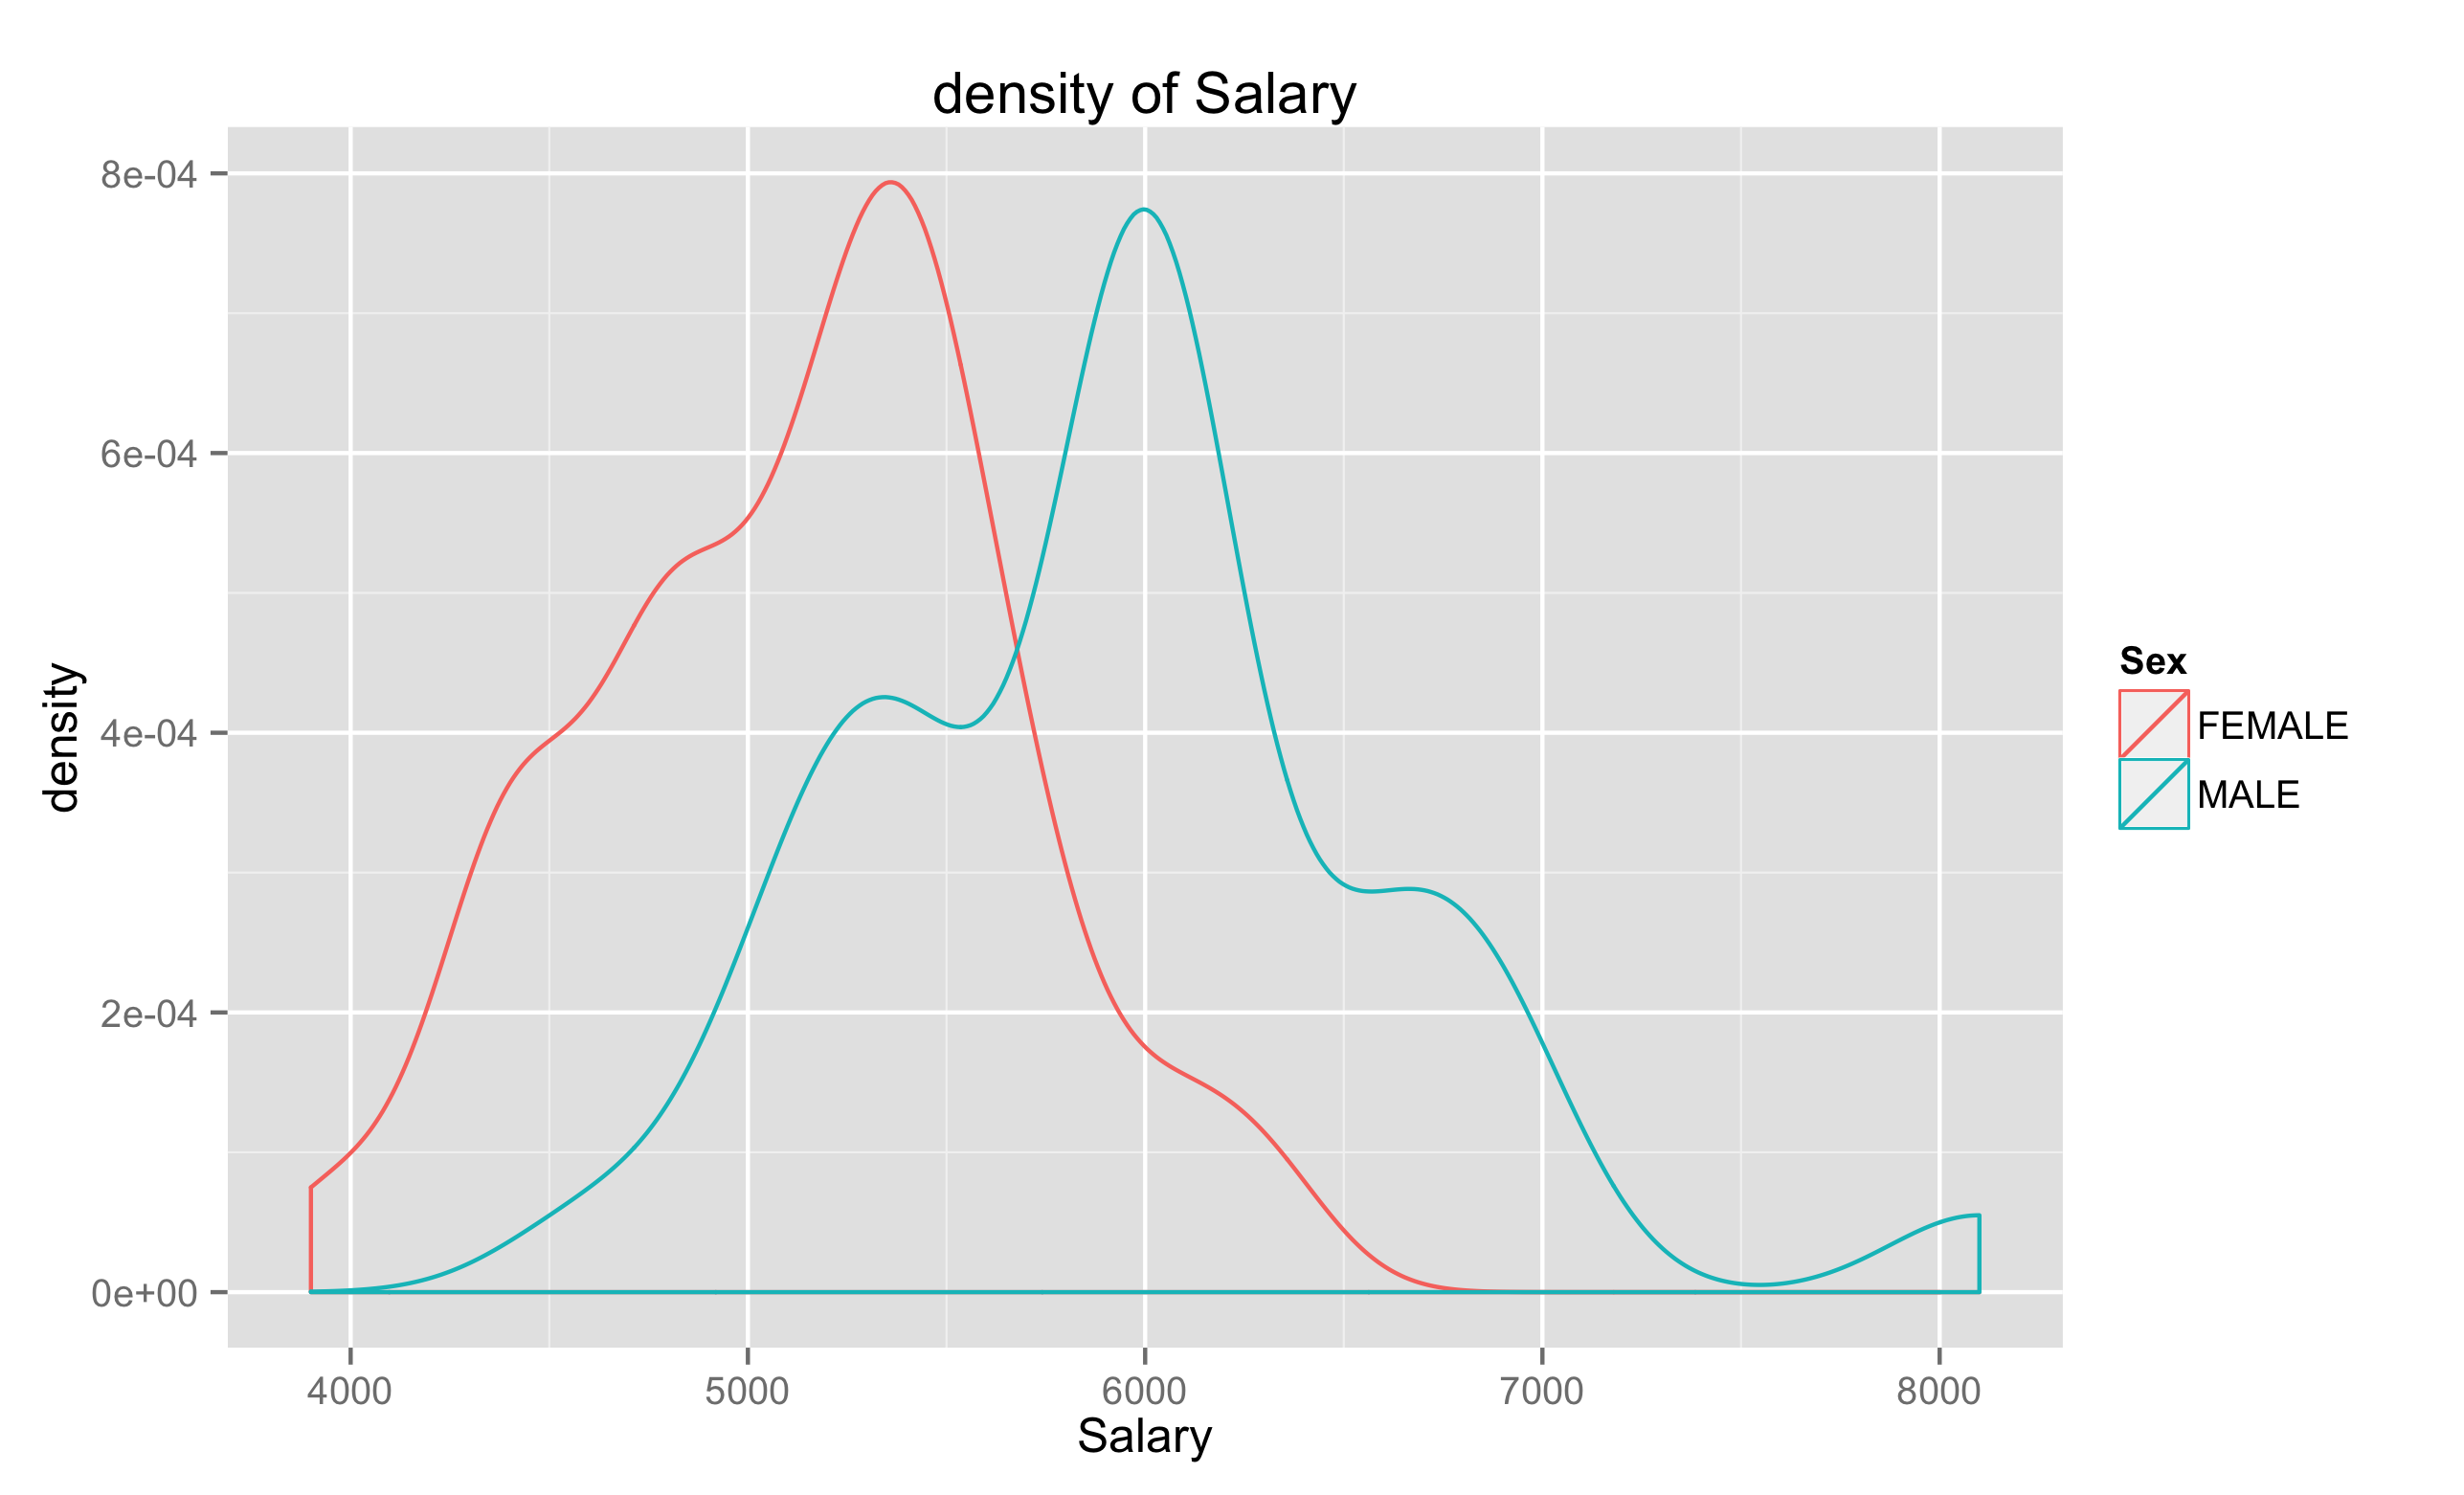
\includegraphics[scale=0.13]{epdf}
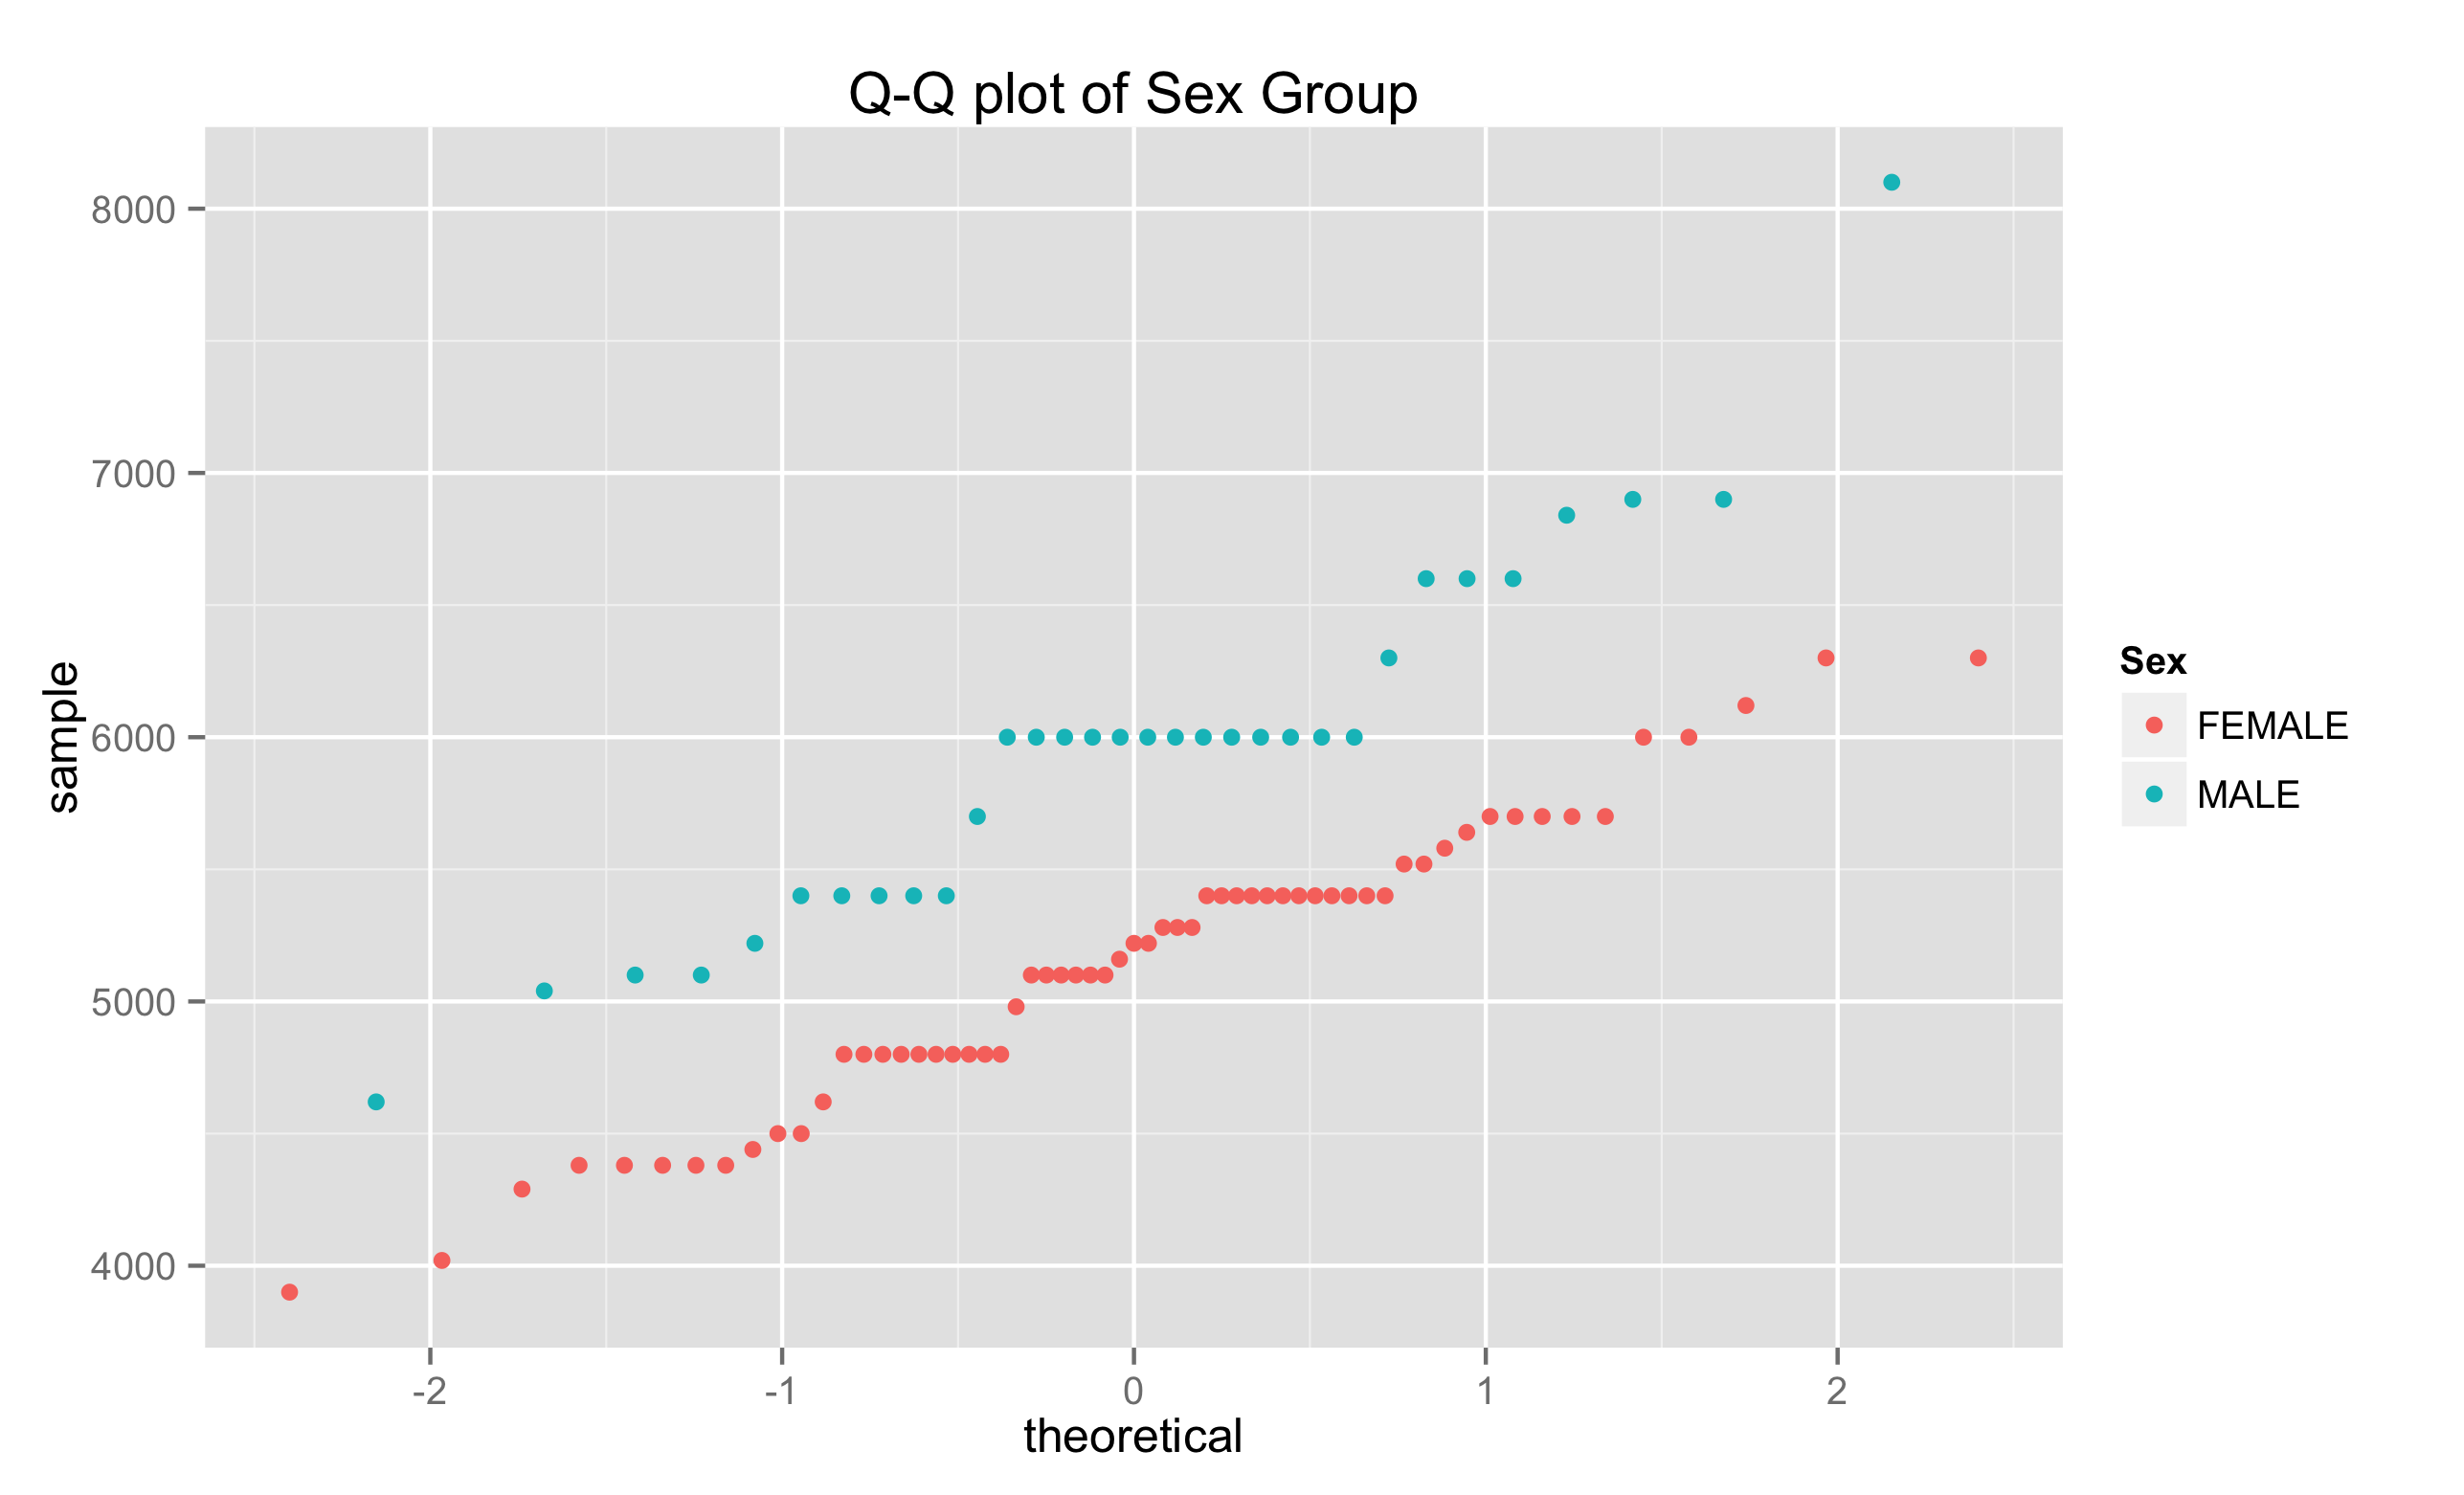
\includegraphics[scale=0.13]{qqplot}
\end{center}

\begin{center}
stem-leaf plot for Male Group
\verbatiminput{stemMale.txt}
\end{center}

\begin{center}
stem-leaf plot for Female Group
\verbatiminput{stemFemale.txt}
\end{center}

\item[\Rmnum{3}). ] For each of the estimates computed in \Rmnum{2} above, determine the bias and variance using each of the following methods (Jackknife, Bootstrap).
\begin{enumerate}[leftmargin=0cm,itemindent=.5cm,labelwidth=\itemindent,labelsep=0cm,align=left]
\item[\textbullet] Jackknife

Using Jackknife method, we calculate the bias and variance of the statistics, including sample mean, median, variance, sd, and IQR. The results are as follows:
\begin{table}[H]
\caption{Jackknife result of bias and variance for MALE}
\centering
\begin{tabular*}{0.8\linewidth}{@{\extracolsep{\fill}}cccccc}

\hline
&Mean & Median & Variance & SD & IQR\\
\hline
bias  & 0 & 0 & 0 & -11.28011& 1162.5\\
\hline
variance & 14909.78 & 0 & 26077372928 & 15578.98 & 130781.2\\
\hline
\end{tabular*}

\caption{Jackknife result of bias and variance for FEMALE}
\centering
\begin{tabular*}{0.8\linewidth}{@{\extracolsep{\fill}}cccccc}
\hline 
&Mean & Median & Variance & SD & IQR\\
\hline
bias  & 0 & -914.7541 & 0 & -1.946738& 0\\
\hline
variance & 4778.038 & 13496.38 & 2401113681 & 2101.91 & 0\\
\hline
\end{tabular*}
\end{table}

\item[\textbullet] Bootstrap

Using Bootstrap method, we calculate the bias and variance of the statistics, including sample mean, median, variance, sd, and IQR. The results are as follows:

\begin{table}[H]
\caption{Bootstrap result of bias and variance for MALE}
\centering
\begin{tabular*}{0.8\linewidth}{@{\extracolsep{\fill}}cccccc}
\hline &Mean & Median & Variance & SD & IQR\\
\hline
bias  & -7.25625 & -9 & -16276.43 & -37.64311& 44.55\\
\hline
variance & 17465.74 & 3100 & 26402928665 & 12611.84 & 89892.98\\
\hline
\end{tabular*}

\caption{Bootstrap result of bias and variance for FEMALE}
\centering
\begin{tabular*}{0.8\linewidth}{@{\extracolsep{\fill}}cccccc}
\hline &Mean & Median & Variance & SD & IQR\\
\hline
bias  & -5.965574 & -14.4 & -2040.152 & -6.274852 & 64.2\\
\hline
variance & 5188.242 & 12008.73 & 2424468372 & 2346.072 & 16673.09\\
\hline
\end{tabular*}
\end{table}

\end{enumerate}
\end{enumerate}
\newpage
\textbf{R Code}:
\begin{lstlisting}
rm(list=ls())

#input raw data file
file<-file("/Users/raymond/Desktop/STAT W4201/HW1/data.txt","r")
data<-readLines(file)
index<-which((1:length(data))%%2==1)
salary<-as.numeric(data[index])
sex<-data[-index]
close(file)
data<-data.frame(Salary=salary,Sex=sex)

#boxplot for the combined data
library(ggplot2)
combined<-ggplot(data,aes("Combined Sex",Salary))
combined+geom_boxplot()+labs(x="Sex",title="Boxplot of combined Salary")
ggsave(file="/Users/raymond/Desktop/STAT W4201/HW1/boxcombined.png")

stem(data$Salary)
sink("/Users/raymond/Desktop/STAT W4201/HW1/stemCombined.txt")
stem(data$Salary)
sink()

#explore if missing values
any(is.na(data$Salary))

#boxplot for Grouped data
Group<-ggplot(data,aes(Sex,Salary))
Group+geom_boxplot()+ggtitle("Boxplot of Salary")
ggsave(file="/Users/raymond/Desktop/STAT W4201/HW1/boxgroup.png")

#stem-leaf plot for Grouped data
stem(data$Salary[data$Sex=="FEMALE"])
stem(data$Salary[data$Sex=="MALE"])
sink("/Users/raymond/Desktop/STAT W4201/HW1/stemFemale.txt")
stem(data$Salary[data$Sex=="FEMALE"])
sink()
sink("/Users/raymond/Desktop/STAT W4201/HW1/stemMale.txt")
stem(data$Salary[data$Sex=="MALE"])
sink()


#scatter plot for Grouped data
Group+geom_point(aes(color=factor(Sex)))+scale_color_discrete(name="Sex")+ggtitle("Scatter of Salary")
ggsave(file="/Users/raymond/Desktop/STAT W4201/HW1/scatter.png")

#histogram for two groups
hist<-ggplot(data,aes(Sex))
hist+geom_histogram()+ggtitle("Histogram of Sex Group")
ggsave(file="/Users/raymond/Desktop/STAT W4201/HW1/histogram.png")
Female<-data$Salary[data$Sex=="FEMALE"]
Male<-data$Salary[data$Sex=="MALE"]
summary(data$Salary[data$Sex=="FEMALE"])
summary(data$Salary[data$Sex=="MALE"])

#estimate density for two groups
epdf<-ggplot(data,aes(Salary))
epdf+geom_density(aes(color=Sex))+ggtitle("density of Salary")
ggsave(file="/Users/raymond/Desktop/STAT W4201/HW1/epdf.png")

#qqplot for two groups
qqplot<-ggplot(data,aes(sample=Salary))
qqplot+stat_qq(aes(color=factor(Sex)))+ggtitle("Q-Q plot of Sex Group")+scale_color_discrete(name="Sex")
ggsave(file="/Users/raymond/Desktop/STAT W4201/HW1/qqplot.png")

#calculate sd for two groups
SD1<-sd(Female)
SD2<-sd(Male)

#jackknife calculate two groups
#MALE group
library(bootstrap)
jmean_Male<-jackknife(Male,mean)
jsd_Male<-jackknife(Male,sd)
jmed_Male<-jackknife(Male,median)
jIQR_Male<-jackknife(Male,IQR)
jvar_Male<-jackknife(Male,var)

#FEMALE group
jmean_Female<-jackknife(Female,mean)
jsd_Female<-jackknife(Female,sd)
jmed_Female<-jackknife(Female,median)
jIQR_Female<-jackknife(Female,IQR)
jvar_Female<-jackknife(Female,var)

#Bootstrap calculate two groups
#MALE group
set.seed(123)
bMeanMale<-bootstrap(Male,100,mean)
bMeanMale_bias<-mean(bMeanMale$thetastar)-mean(Male)
bMeanMale_var<-var(bMeanMale$thetastar)
bMedMale<-bootstrap(Male,100,median)
bMedMale_bias<-mean(bMedMale$thetastar)-median(Male)
bMedMale_var<-var(bMedMale$thetastar)
bsdMale<-bootstrap(Male,100,sd)
bsdMale_bias<-mean(bsdMale$thetastar)-sd(Male)
bsdMale_var<-var(bsdMale$thetastar)
bvarMale<-bootstrap(Male,100,var)
bvarMale_bias<-mean(bvarMale$thetastar)-var(Male)
bvarMale_var<-var(bvarMale$thetastar)
bIQRMale<-bootstrap(Male,100,IQR)
bIQRMale_bias<-mean(bIQRMale$thetastar)-IQR(Male)
bIQRMale_var<-var(bIQRMale$thetastar)

#FEMALE Group
bMeanFemale<-bootstrap(Female,100,mean)
bMeanFemale_bias<-mean(bMeanFemale$thetastar)-mean(Female)
bMeanFemale_var<-var(bMeanFemale$thetastar)
bMedFemale<-bootstrap(Female,100,median)
bMedFemale_bias<-mean(bMedFemale$thetastar)-median(Female)
bMedFemale_var<-var(bMedFemale$thetastar)
bsdFemale<-bootstrap(Female,100,sd)
bsdFemale_bias<-mean(bsdFemale$thetastar)-sd(Female)
bsdFemale_var<-var(bsdFemale$thetastar)
bvarFemale<-bootstrap(Female,100,var)
bvarFemale_bias<-mean(bvarFemale$thetastar)-var(Female)
bvarFemale_var<-var(bvarFemale$thetastar)
bIQRFemale<-bootstrap(Female,100,IQR)
bIQRFemale_bias<-mean(bIQRFemale$thetastar)-IQR(Female)
bIQRFemale_var<-var(bIQRFemale$thetastar)

\end{lstlisting}
\end{document}